%!TEX root = bertini_real_manual.tex

\section{Installation}
\label{sec:installation}


This section of the manual focuses on how to install the necessary dependencies and programs needed to run Bertini\_real on a user's computer. The instructions provided describe the process for Linux, Mac, and Windows operating systems.  If you need help or encounter an problem, please file an issue \href{https://github.com/ofloveandhate/bertini_real/issues}{on Github}; this is much preferred over email.

When installing Bertini\_real, there are a number of steps required in order to successfully install and run the program. They are:
\begin{enumerate}
\item Installing the \glspl{dependent}
\item Installing Bertini
\item Installing Bertini\_real
\end{enumerate}




\subsection{Dependencies}
\label{sec:deps}

Before installing Bertini 1 and then Bertini\_real, there are a number of packages that need to be installed. The method used to install these \glspl{dependent} changes depending on the operating system, so please be sure to read the section that describes your particular system.  Except for Bertini, you should be able to install all of these using a package manager.  It's there to help.

\paragraph{Bertini 1 dependencies}

\begin{itemize}[noitemsep]
\item \gls{mpfr}
\item \gls{gmp}
\item MPI (whatever implementation you want)
\item flex
\item bison
\end{itemize}


\paragraph{Bertini\_real dependencies}

\begin{itemize}[noitemsep]
\item a C++ compiler capable of the C++14 standard
\item Bertini 1, {\bf parallel version compiled from source and installed as library}.
\item \gls{mpi} (Must be the same one as Bertini was compiled with)
\item Boost $>$= 1.53
\item For Bertini\_real versions 1.8.x and before, {\tt autoconf}, {\tt automake}, {\tt make}, {\tt libtool}.  
\item For Bertini\_real versions 1.9 and later {\tt cmake}
\end{itemize} 



Bertini\_real is parallel-enabled, using MPI.  {\bf You cannot build Bertini\_real without support for MPI at the current time, and so you must also have parallel Bertini 1 installed as a library}.  To use multiple processors to decompose a real object, call Bertini\_real as you would any other MPI program: \texttt{mpiexec [options] bertini\_real [options]}.  It also works in serial, without being hosted by the MPI executor.  But you still have to have MPI to build it.  


\subsubsection{Symbolic engine}

One additional piece of software must be installed in order to decompose surfaces -- something to do symbolic work for us (Bertini does not include a symbolic engine).  Two options are available:  Matlab, and Python.  The Matlab suite has much stronger visualization routines for Bertini\_real.  But Python is free!  Python is the default engine.

	\paragraph*{MATLAB}
One option for symbolic engine for Bertini\_real is Matlab.  Instructions on how to install the program are not provided here. However, if you are associated with a university, or a research facility, they probably have download instructions on their technology support website.   Ensure you have access to the symbolic toolbox.  It's required.

You must add Matlab to the terminal path -- you have to be able to type {\tt matlab} into a terminal and have it launch.  

If you intend to use Matlab for visualization, you need to add {\tt path/to/bertini\_real/matlab\_codes} to the path, as well as several folders in there, namely {\tt matlab\_codes/brakelab/bertini1} and {\tt matlab\_codes/brakelab/rendering}

\paragraph*{Python}

Bertini\_real was improved in Fall 2016 to allow you to use Python as the symbolic engine, in alternative to Matlab.  This allows for fully free software to do the decompositions.  

You need the following packages, ideally from {\tt pip}:
\begin{itemize}[noitemsep]
\item {\tt sympy}
\item {\tt scipy}
\item {\tt numpy}
\item {\tt algopy}
\item {\tt mpmath}
  \end{itemize}
and for visualization
\begin{itemize}[noitemsep]
\item {\tt dill}
\item {\tt matplotlib}
  \end{itemize}






\clearpage
%!TEX root = bertini_real_manual.tex

\subsection{Instructions for GNU/Linux}
\label{sec:install_linux}


These instructions were last updated in July 2025.


\begin{enumerate}
\item Install dependencies. You are very strongly encouraged to use the package manager provided, such as {\tt apt} or {\tt yum}, to install the dependencies.  See Section~\ref{sec:deps} for a list of dependencies.
\item Build and install Bertini1, ensuring that you are building the parallel version.  You must install from source, simply downloading the pre-built executable will not get you the built libraries.

\begin{enumerate}
	\item Move to the source directory
	\item For Bertini versions 1.6.x and before,
	\begin{enumerate}
		\item {\tt ./configure}
		\item {\tt make -j 4}
		\item {\tt sudo make install}
	\end{enumerate}
	\item For Bertini1 versions 1.7.x and later, 
      \begin{enumerate}
        \item \verb|mkdir build && cd build|
        \item \verb|cmake ../|
        \item \verb|make -j 4|
        \item \verb|make install| \\ Installing may require \verb|sudo|
      \end{enumerate}

\end{enumerate}
\item Build and install Bertini\_real.  
\begin{enumerate}
	\item Clone from repo, {\tt git clone https://github.com/ofloveandhate/bertini\_real}.  

	\item Move to the directory.

	\item For versions 1.8.x and before,
	\begin{enumerate}
		\item {\tt libtoolize}
		\item {\tt autoreconf -i} \quad if you know how to eliminate these steps by writing a bootstrap file which works on all systems, please contribute by way of a pull request.  PR's gladly acccepted to {\tt develop}.
		\item {\tt ./configure}
		\item {\tt make -j 4}
		\item {\tt sudo make install}
	\end{enumerate}

	\item For Bertini\_real 1.9 and later, using cmake:
	\begin{enumerate}
	  \item \verb|mkdir build && cd build|
	  \item \verb|cmake ../|
	  \item \verb|make -j 4|
	  \item \verb|make install| \\ Installing may require \verb|sudo|
	\end{enumerate}

	\item eat something delicious, and give thanks for this peaceful day
\end{enumerate}
\item[*]
If using Matlab for symbolic engine, ensure it is installed an on the path for the command line.  In bash, \verb|export PATH=$PATH:/PATH/TO/MATLAB/bin|, and you can place this in \verb|.bash_profile| perhaps.%
\footnote{Note that there are several possible files into which to place this, and this particular method of using {\tt export} is shell specific.  The {\tt csh} is a little different, for example.  Too lazy to Google it?  I gotcha: \href{https://www.google.com/\#q=add+to+path+linux&*}{search on da googs here} } 

\item[*]
If using Python for symbolic engine, install your favorite version, {\tt pip}, and the necessary modules via {\tt pip}.

\end{enumerate}


If anything went wrong, please file an issue \href{https://github.com/ofloveandhate/bertini_real/issues}{on Github}.  I want this to be an easy experience.


\clearpage
%!TEX root = bertini_real_manual.tex

\subsection{Instructions for OSX}

These instructions were last updated in July 2025.


\subsubsection{Preliminary Work}
\begin{itemize}
  \item Compilers \&c: In terminal, type {\tt xcode-select --install}
   
  \item Homebrew: It is highly recommended that Mac users install the program \href{http://brew.sh}{Homebrew} to use to install these packages. Once that has been done, installing the previously listed dependencies becomes simple. In terminal,  type \texttt{brew search \_\_\_\_} to list packages related to \_\_\_\_, where \_\_\_\_ is your search (for example, GMP, Boost, or MPI). To download new software via Homebrew, type in terminal \texttt{brew install \_\_\_\_} 

  Suggested call:

  \texttt{brew install cmake autoconf automake libtool mpfr gmp mpich boost}
   \item Matlab: make sure to have it installed, and on the path for the command line.
   \item Python: use {\tt pip} to install dependencies
\end{itemize}


\subsubsection{Build and install Bertini 1}

\begin{enumerate}
  \item Download the source tarball ({\tt .tar.gz}) from \href{http://bertini.nd.edu}{bertini.nd.edu}
  \item Unpack the tarball (just double click it, if you're into mousing)
  \item If you didn't already, now use Homebrew to install the dependencies for Bertini1 \\{\tt brew install cmake autoconf automake libtool mpfr gmp mpich boost}\\ (Bertini1 doesn't depend on Boost, but Bertini\_real does)
  \item In the terminal, move to the unpacked folder for Bertini 1

  \item Compile.
  \begin{enumerate}

    \item For Bertini versions 1.6.x and before, use the make build system, using this classic pattern:
    \begin{enumerate}
      \item {\tt ./configure}.  \\ If you're using homebrew, this may require \\ \verb|./configure LDFLAGS=-L/opt/homebrew/lib CPPFLAGS=-I/opt/homebrew/include| 
      \item {\tt make -j 4 \&\& make install}\\ installing may require \verb|sudo|
    \end{enumerate}

    \item For Bertini versions 1.7 and later, use CMake.
      \begin{enumerate}
        \item \verb|mkdir build && cd build|
        \item \verb|cmake ../|
        \item \verb|make -j 4|
        \item \verb|make install| \\ Installing may require \verb|sudo|
      \end{enumerate}
  \end{enumerate}
\end{enumerate}

\subsubsection{Build and install Bertini\_real}

\begin{enumerate}
  \item Clone the repo to get the code.
  \begin{enumerate}
    \item {\tt which git}  if it's emtpy, then {\tt brew install git}
    \item {\tt mkdir code \&\& cd code}
    \item {\tt git clone https://github.com/ofloveandhate/bertini\_real}
  \end{enumerate}

  \item Move into the directory.  {\tt cd bertini\_real}

  \item Compile using one of two options
    \begin{enumerate}
      \item For Bertini\_real 1.8 and before, using the classic make system:
      \begin{enumerate}
        \item {\tt autoreconf -i}
        \item {\tt ./configure}
        \item {\tt make -j 4 \&\& make install} Installing may require \verb|sudo|
      \end{enumerate} 

      \item For Bertini\_real 1.9 and later, using cmake:
      \begin{enumerate}
        \item \verb|mkdir build && cd build|
        \item \verb|cmake ../|
        \item \verb|make -j 4|
        \item \verb|make install| \\ Installing may require \verb|sudo|
      \end{enumerate}


    \end{enumerate}

\end{enumerate}


Problems?  Raise an issue \href{https://github.com/ofloveandhate/bertini_real/issues}{on Github}, please. 


\clearpage
%!TEX root = bertini_real_manual.tex

\subsection{Instructions for Windows}


Bertini is currently not working on Windows, even in Cygwin, because I have been struggling to get it to find MPI while configuring using CMake.   These instructions are not correct, but {\em they should be}, if I could get CMake to find OpenMPI in Cygwin...  Someone help?

---

\begin{enumerate}

\item Install Cygwin.  \url{https://www.cygwin.com/}  Download the installer (3.6.4)  \url{https://www.cygwin.com/install.html}. Run the installer. Click click!

\item Install packages inside of Cygwin.  (If you later need to install more packages after you install Cygwin, just use the same installer you used to install Cygwin in the first place.)
Use the search tool, having selected "full" from the dropdown.  Locate the package, and select the most recent version using the dropdown.  Then check the checkbox.

\begin{itemize}
\item libgmp-devel
\item libmpfr-devel
\item cmake (3.31 is good, though it's marked as test)
\item flex
\item bison
\item gcc-core (i used 13.4.1, because later versions were marked test
\item make 
\item OpenMPI
\end{itemize}

Finally, click through to install.  It will download and install things.

\item Download and extract the contents of the zip for the source of Bertini 1.7.  Copy the source folder to your folder in the cygdrive.  For me, it's at \verb|C:\cygwin64\home\amethyst|.  I put the source directory at the level of my home folder (inside Cygwin).

\item In the Cygwin64 terminal

\begin{enumerate}
   \item cd into the source directory
   \item mkdir build
   \item cd build
   \item cmake ../ 
   \item make -j 4
   \item make install
\end{enumerate}

\end{enumerate}






















\clearpage

\subsection{Testrun -- the Cayley Cubic}

Now that everything has been installed, we can now do a test run, to make sure that everything is working properly. To test this program, we will try to generate a Cayley Cubic using the above programs, following a number of steps. The first step is to create an input file. Open up a text editor in your terminal and create a file called \texttt{input}. 

Below is the text for this input file.  A key feature to notice is the second line, where the \texttt{tracktype} configuration is set to {\tt 1}. This configuration setting is necessary for Bertini to run, to run the needed {\tt witness\_data} file that Bertini\_real uses as input. 

\begin{center}\begin{minipage}{0.9\linewidth}
\begin{lstlisting}[language=c++, caption={\tt input} for the Cayley Cubic, captionpos=b]
CONFIG 
tracktype:1;

END;
INPUT
variable_group x, y, z;
function f;
f = 4 * (x^2 + y^2 + z^2) + 16*x*y*z - 1;
END;
\end{lstlisting}
\end{minipage}\end{center}

Once the input file is created, we can now run Bertini. Simply navigate in the command line to the directory of the input file and type \texttt{bertini} or \texttt{bertini input}.%
\footnote{Depending on how you installed Bertini\_real, you may need to type in the entire path to where Bertini is located, if it's not in the same folder, so the command line read \newline \texttt{/cygdrive/path/to/BertiniSource\_v1.6/bertini-serial.exe input} \textbf{Cygwin users:} For Bertini versions 1.6.x and before, a user may also use \texttt{bertini-serial.exe} (or \texttt{bertini\_parallel.exe}). }  
This will run Bertini, creating the Numerical Irreducible Decomposition needed for Bertini\_real. Something like the following should print to the screen:


\begin{center}\begin{minipage}{0.9\linewidth}
\centering
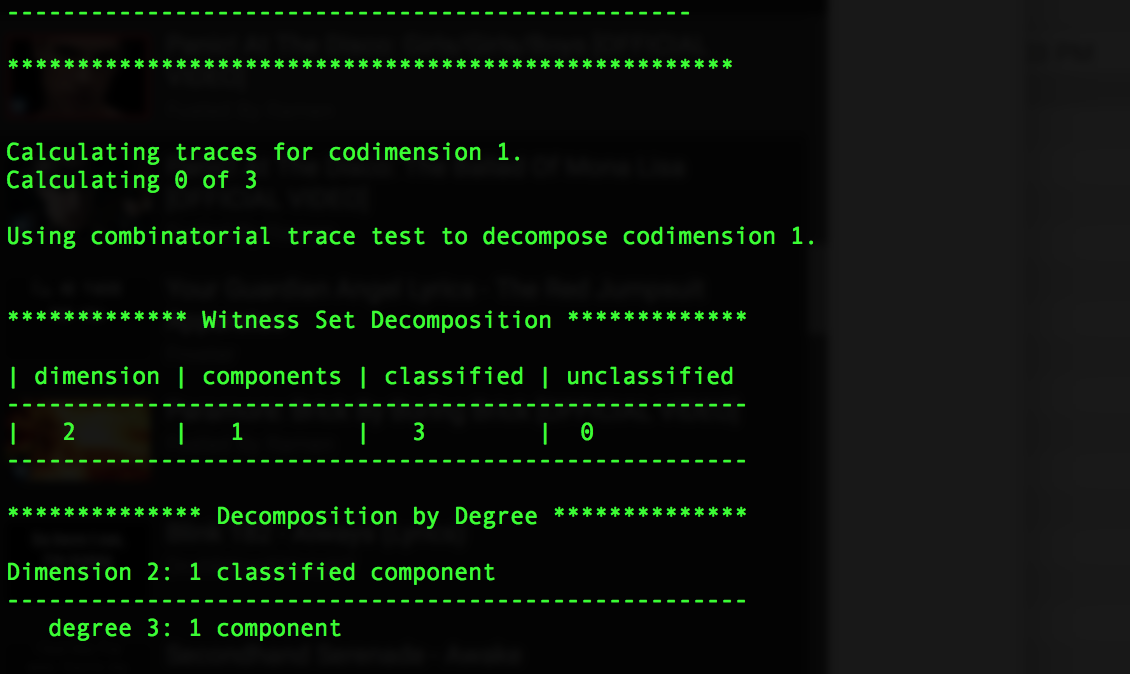
\includegraphics[width=0.6\textwidth]{CayleyCubicBertiniRun.png}
\end{minipage}\end{center}

Once Bertini is finished with the NID, the output can be verified as satisfactory (or not). 

Bertini\_real can be run by calling \texttt{bertini\_real} in the command line.%
\footnote{Cygwin users, the same rules that applied to Bertini also apply to Bertini\_real, so be sure to include that `.exe' at the end!}
This program should run for roughly 20-30 seconds (ymmv), with the final terminal/shell output appearing below:

\begin{center}\begin{minipage}{0.9\linewidth}
\centering
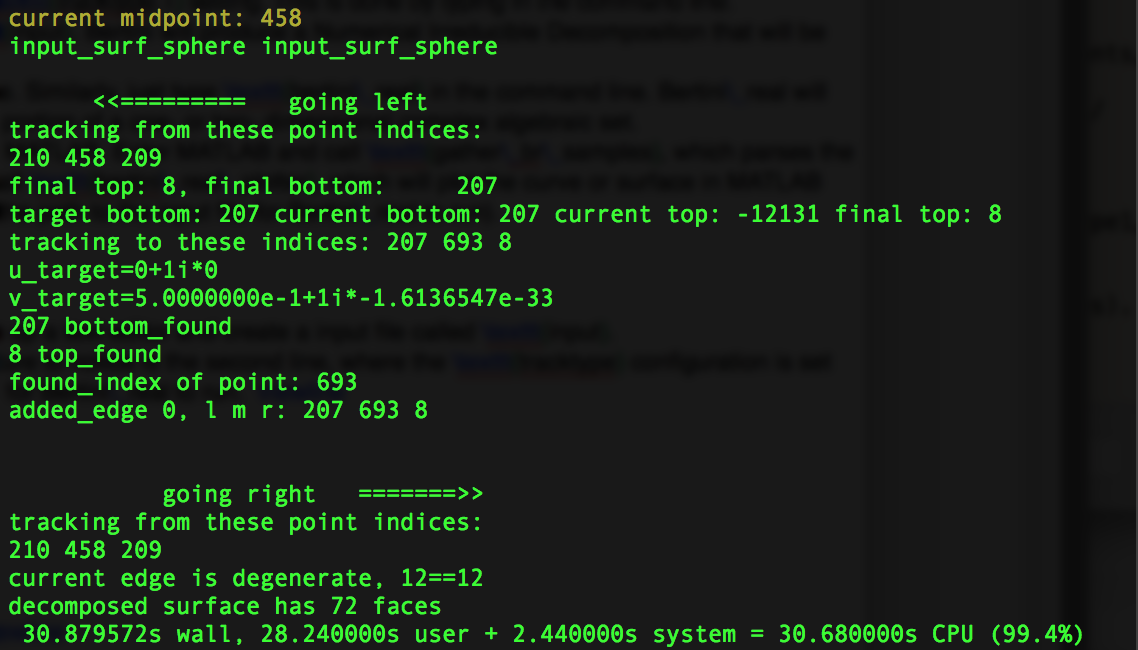
\includegraphics[width=0.6\textwidth]{CayleyCubicBertiniRealRun}
\end{minipage}\end{center}

Finally, we can visualize.  I'm assuming here you're using Matlab -- see elsewhere in this manual for Python instructions.  Make sure that the \verb|matlab_codes| folder inside the \verb|bertini_real| repo is added to the path, with subfolders.  

\begin{enumerate}
  \item Open MATLAB and move to the folder for the surface.  
  \item Call \texttt{gather\_br\_samples} in the command window.  This generates a \verb|BRinfo*.mat| file, sequentially numbered so as to not overwrite previous results.
  \item Run \texttt{bertini\_real\_plotter\-}. This loads the highest-numbered data files, and creates create a MATLAB figure, pictured below.  In-figure controls let you modify and save the figure.
\end{enumerate}

\begin{center}\begin{minipage}{0.9\linewidth}
\centering
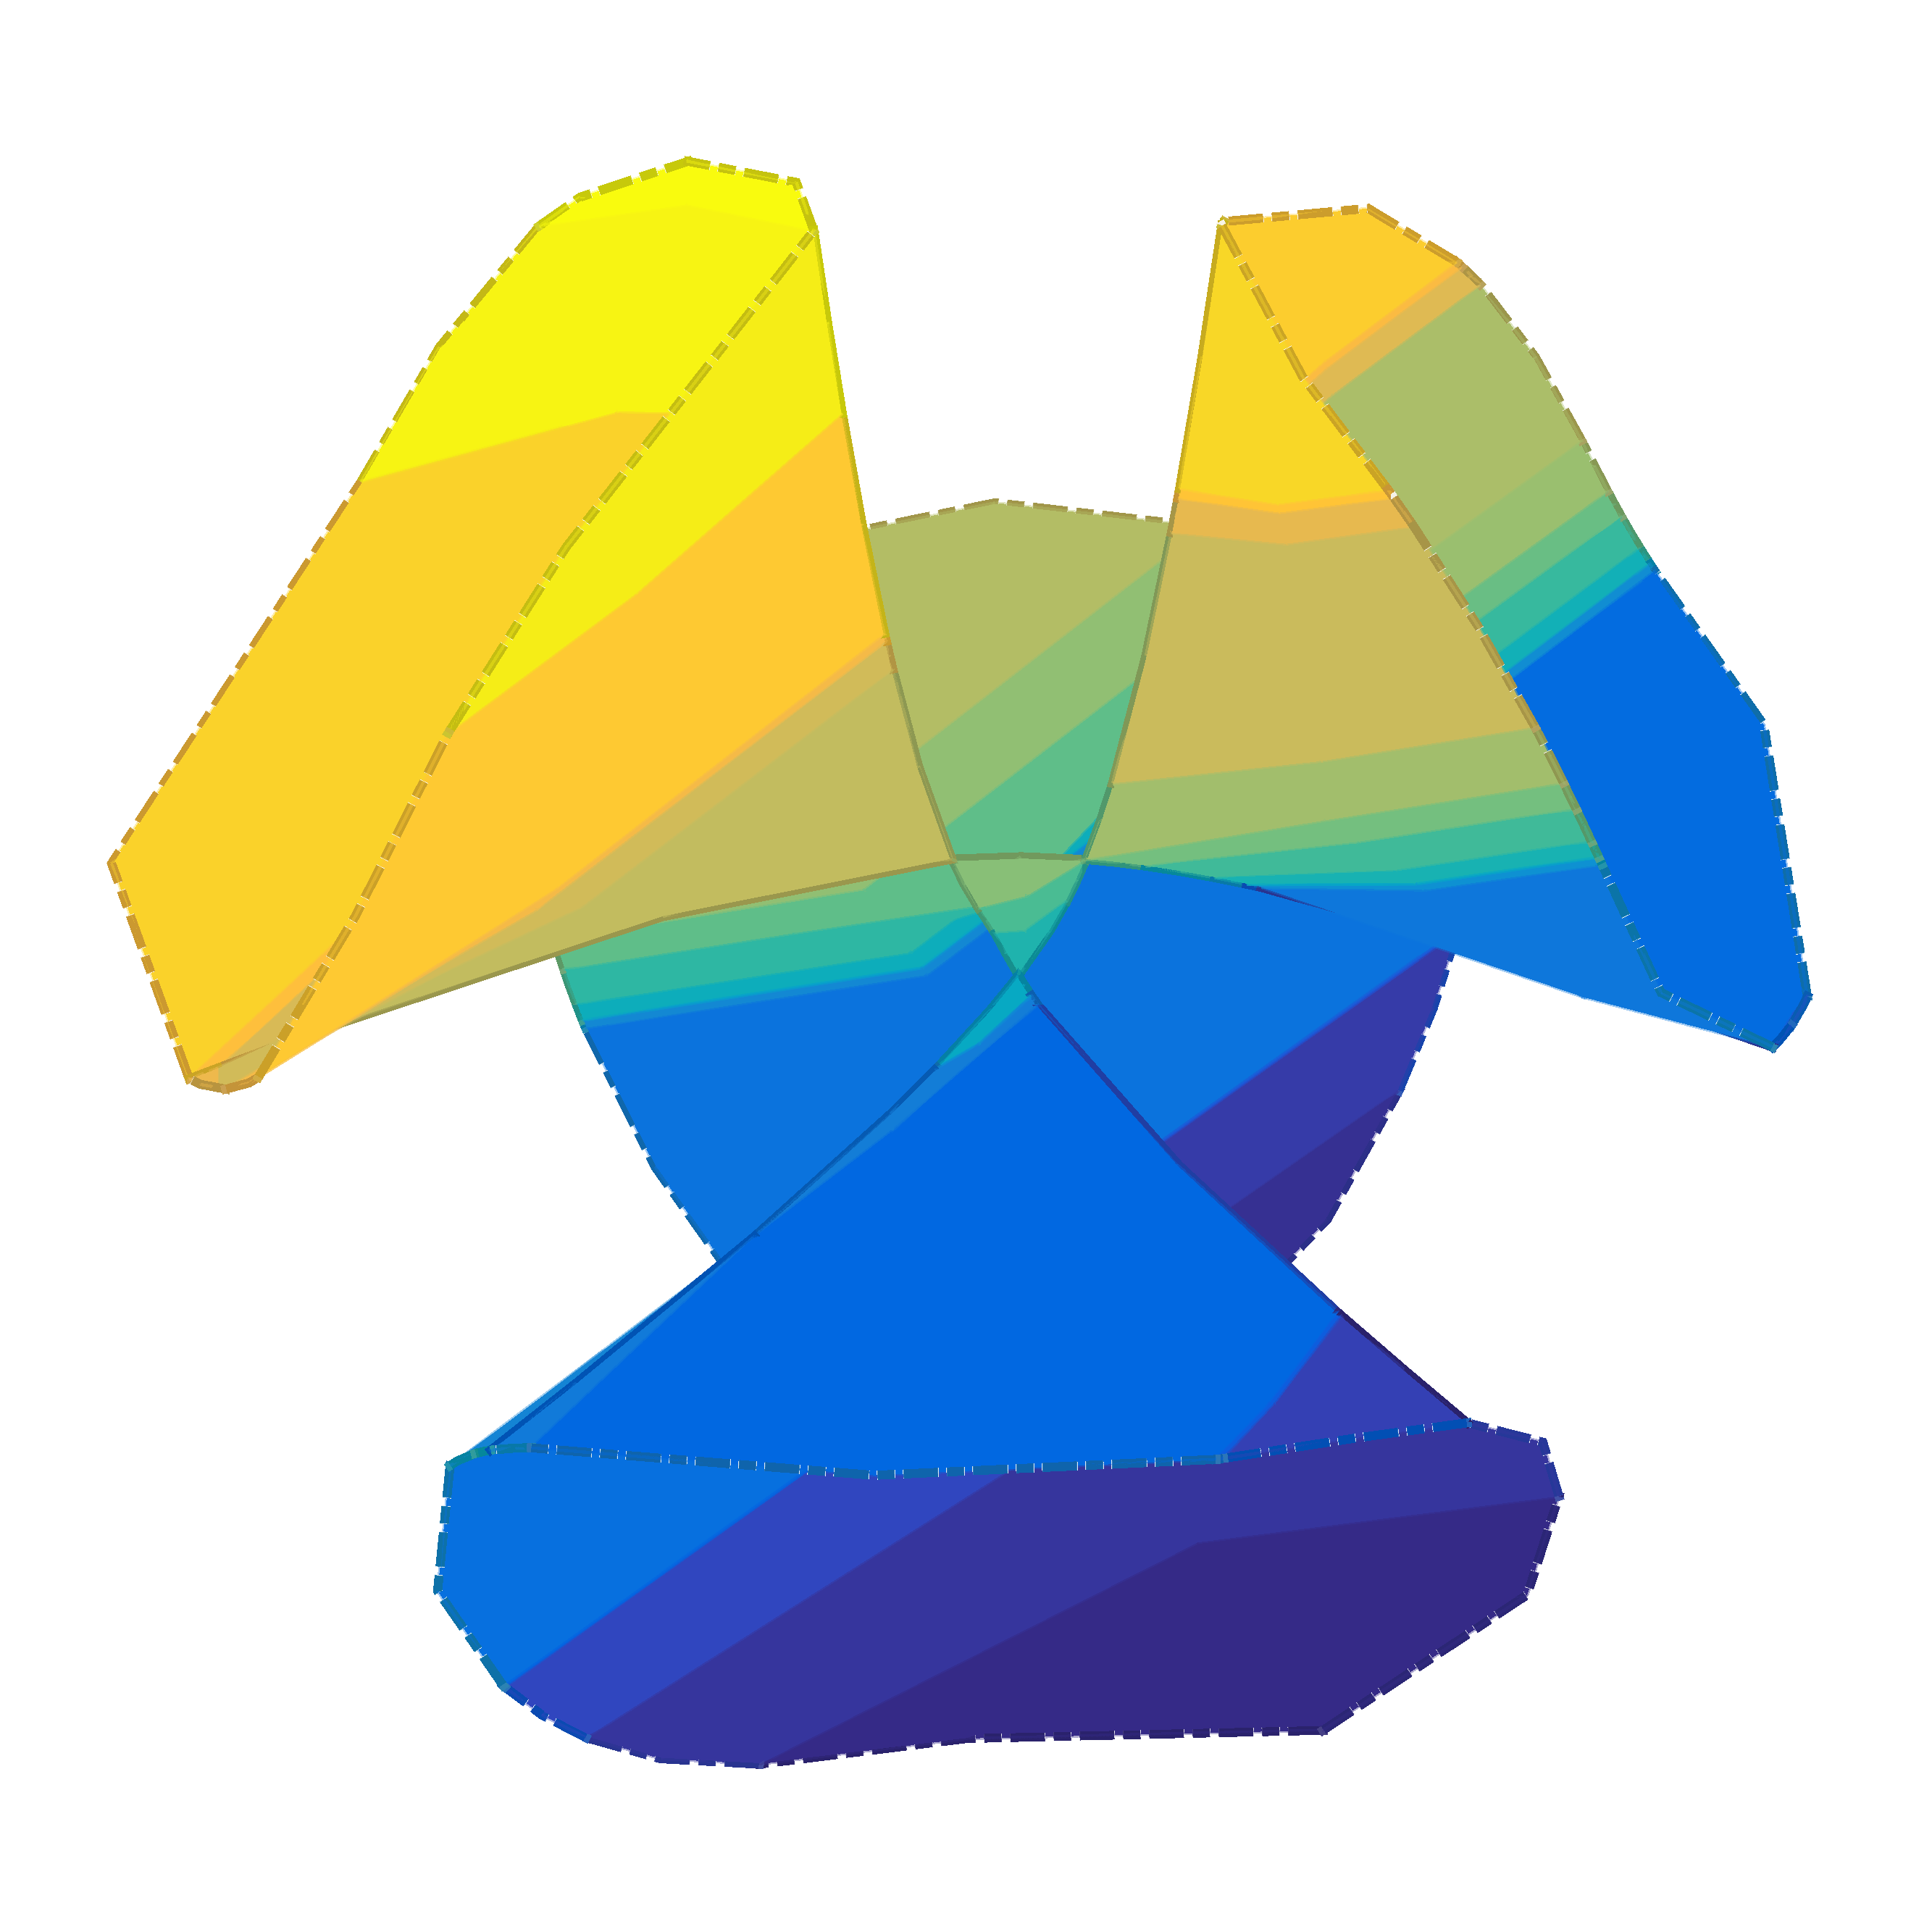
\includegraphics[width=0.6\textwidth]{CayleyCubic}
\end{minipage}\end{center}


If you've been able to reproduce the above figure, then you've mastered the basics of Bertini\_real. 





